\documentclass[a4paper,12pt]{article}

% Use pdfLaTeX for Cyrillic support
\usepackage[utf8]{inputenc}
\usepackage[T2A]{fontenc}
% Remove babel bulgarian to avoid incompatibility
% \usepackage[bulgarian]{babel} % Language support

\usepackage{amsmath, amssymb}
\usepackage{listings}
\usepackage{xcolor}
\usepackage{url}
\usepackage{graphicx}
%Comments
\usepackage{pdfcomment}

% Define colors similar to Pygments/minted
\definecolor{codegreen}{rgb}{0,0.6,0}
\definecolor{codegray}{rgb}{0.5,0.5,0.5}
\definecolor{codepurple}{rgb}{0.58,0,0.82}

\definecolor{backcolour}{rgb}{0.95,0.95,0.92}

% Listing style
\lstset{
    commentstyle=\color{codegreen},
    keywordstyle=\color{magenta},
    numberstyle=\tiny\color{codegray},
    stringstyle=\color{codepurple},
    basicstyle=\ttfamily\footnotesize,
    breakatwhitespace=false,         
    breaklines=true,                 
    captionpos=b,                    
    keepspaces=true,                 
    numbers=left,                    
    numbersep=5pt,                  
    showspaces=false,                
    showstringspaces=false,
    showtabs=false,                  
    tabsize=2,
    frame=none,
}




\title{\textbf{Дисертация на тема
        \\[0.5em] \large{Разработване на виртуална среда за актюерски пенсионни изчисления}}}
\author{Георги Веселинов Бурнаски
        \\ Катедра Mагистърска програма- Вероятности актюерство и статистика
        \\ Факултет по Математика и Информатика
        \\ Софийски Университет "Св. Климент Охридски"}
\date{\today}

\begin{document}
\maketitle
\newpage
\section{Увод}
Актюерската математика заема все по-значимо място в съвременното общество, където управлението на финансовите рискове и дългосрочната устойчивост на социалните системи са от първостепенно значение.

В условията на застаряващо население, динамични финансови пазари и нарастващи изисквания към пенсионните системи, надеждните и прецизни актюерски изчисления се превръщат в ключов инструмент за вземане на информирани решения. Те подпомагат както държавните институции при моделиране и реформиране на пенсионните схеми, така и частните компании при разработване на застрахователни и инвестиционни продукти \cite{dalriada2023}.

Актюерските методи намират широко приложение в различни сфери:
пенсионното осигуряване, животозастраховането здравното застраховане, управлението на фондове и финансовото планиране. Общото между всички тези области е необходимостта от точни прогнози, основани на статистически модели и вероятностни методи, които да оценяват бъдещи парични потоци, продължителност на живота и свързаните с тях рискове \cite{milliman2022}.

В наши дни пенсионните системи се изправят пред редица сериозни предизвикателства. Демографските промени, и по-специално увеличаването на средната продължителност на живота и намаляването на раждаемостта, водят до нарастващо съотношение между пенсионери и
активно работещо население \cite{bostonfed1999}. Това поставя под натиск публичните пенсионни фондове и създава необходимост от по-прецизни модели за оценка на бъдещите задължения. Паралелно с това колебанията на финансовите пазари и инфлационните процеси влияят върху доходността на пенсионните активи и изискват по-гъвкави подходи при управлението на риска \cite{ncpers2023}.

Съвременните технологии и програмни езици като Python предлагат нови възможности за прилагане на актюерската математика в практиката. Разработването на специализирана библиотека за пенсионни актюерски изчисления има двойна значимост: от една страна, улеснява изследователите и практиците при прилагането на сложни модели, а от друга – допринася за повишаване на прозрачността, възпроизводимостта и достъпността на тези изчисления \cite{lifelib2024, hyperexponential2023}.

Въпреки наличието на различни софтуерни решения за актюерски изчисления, много от тях са или твърде специализирани, или не предлагат необходимата гъвкавост и интеграция с други аналитични инструменти. Python, с богатия си екосистем от библиотеки за научни изчисления и машинно обучение, се явява като идеална платформа за разработване на такава библиотека. Тя би могла да обедини теоретичните основи на актюерската математика с практическите нужди на потребителите, предоставяйки лесен за използване и разширяем инструмент \cite{numpy2024, pandas2024}.

Разработването на библиотека за пенсионни актюерски изчисления в Python би могло да включва функции за изчисляване на настояща стойност на бъдещи парични потоци, моделиране на демографски и финансови рискове, симулации на сценарии и оптимизация на пенсионни стратегии. Освен това, интеграцията с други библиотеки за визуализация и анализ би позволила по-добро представяне и интерпретация на резултатите \cite{matplotlib2024, seaborn2024}.

В заключение, създаването на специализирана библиотека за пенсионни актюерски изчисления в Python представлява важна стъпка към модернизацията и усъвършенстването на актюерската практика. Тя би могла да подпомогне както академичните изследвания, така и практическите приложения, като предостави мощен и достъпен инструмент за анализ и управление на пенсионните системи в съвременния свят.

Пенсионната система в България следва модела на много развити страни и се състои
от три компонента, известни като "трите стълба":
\begin{itemize}
        \item Първи стълб: Държавно задължително пенсионно осигуряване (солидарност между поколенията). Това е държавната пенсия, която се финансира от текущите осигурителни вноски на работещите. Тя е задължителна за всички работещи.
        \item Втори стълб: Допълнително задължително пенсионно осигуряване (ДЗПО). Това е индивидуално натрупване на средства в избрани от самия осигурено лице пенсионни фондове. Той също е задължителен за хората, родени след 31.12.1959 г., които не са избрали да останат само в Първи стълб.
        \item Трети стълб: Допълнително доброволно пенсионно осигуряване (ДДПО). Това е напълно доброволно допълнително пенсионно осигуряване, при което хората сами решават да спестяват допълнително за своята пенсия.
\end{itemize}
В този труд ще се фокусираме върху изчисленията, свързани със втори и трети стълб от пенсионносигурителната система, тъй като те са поети от частните пенсионноосигурителни дружества. В България 20\% от доходите на работещите се отделят за пенсионно осигуряване, като 12.8\% отиват за първи стълб, а 5\% - за втори стълб. Важно е да се отбележи, че тези проценти могат да варират в зависимост от законодателството и икономическите условия. Останалите 2.2\% са за здравно осигуряване и трудови злополуки.\cite{ZDZPO_2004, ZDOO_2000}

Условията за пенсионните изчисления са регламентирани от различни нормативни актове, като основните от тях са:
\begin{itemize}
        \item Кодекс за социално осигуряване (КСО)
        \item Закон за допълнително задължително пенсионно осигуряване (ЗДЗПО)
        \item Закон за допълнително доброволно пенсионно осигуряване (ЗДОО)
        \item Наредба № Н-8 от 2004 г. за определяне на методиката за изчисляване на пенсиите
        \item Наредба № 3 от 2003 г. за условията и реда за изплащане на пенсиите от частните пенсионни фондове
\end{itemize}
Като изчисленията трябва да отговарят на изискванията, заложени наредба 69 от 2003 г. за определяне на методиката за изчисляване на пенсиите от частните пенсионни фондове. \cite{ZDZPO_2004,ZDOO_2000,DKFN_Pensions,NOI_Official}

Целта на настоящата дисертация е именно изграждането на такава библиотека, която да обедини теоретичните основи на пенсионната математика с предимствата на съвременните програмни среди. Чрез нея се цели създаването на гъвкав инструмент, който да подкрепя както научната работа, така и практическите решения в областта на пенсионното осигуряване.
\newpage
\section{Математика}
\subsection{Вероятност за смърт}
Вероятността за смърт $q_x$ е вероятността човек на възраст $x$ да умре преди да достигне възраст $x+1$. Тази вероятност се взима от статистическата статистика на държавната осигурителна институция  в случая Националният осигурителен институт(НОИ)
\subsection{Вероятност за преживяване}
Вероятността за преживяване $p_x= 1-q_x$ е вероятността човек на възраст $x$ да оцелее до следващата година, т.е. до възраст $x+1$.
\subsection{Среден брой живи хора}
Средният брой живи хора на възраст $x$ се обозначава с $l_x$ и представлява броя на хората, които са живи на тази възраст в дадена популация. Тази стойност се използва за изчисляване на вероятността за смърт и други актюерски изчисления. Изчислява се по формулата:
\[l_{x} = l_0 \cdot \prod_{i=0}^{x-1} p_i\]
където $l_0$ е началният брой живи хора (на възраст 0), а $p_i$ е вероятността за преживяване на възраст $i$ и $l_x$ е броят на живите хора на възраст $x$.
\subsection{Дисконтиращ фактор}
Дисконтиращият фактор $v$ се използва за изчисляване на настоящата стойност на бъдещи парични потоци. Той се изчислява по формулата:
\[v = \frac{1}{1+i}\]
където $i$ е годишният лихвен процент зададен от пенсионноосигурителната компания. В нашият случай ще използваме техническия лихвен процент на пенсионна компания "Съгласие" който е 0.15\% \cite{DKFN_Pensions}
\subsection{Настояща стойност}
Настоящата стойност ($D_x$) на бъдещ паричен поток се изчислява чрез дисконтиране на този поток към настоящия момент. Формулата за изчисляване на настоящата стойност е:
\[D_x = l_x\cdot v^x\]
\subsection{Кумулативна настояща стойност}
Кумулативната настояща стойност ($N_x$) представлява сумата от настоящите стойности на всички бъдещи плащания за период от $n$ години. Тя се изчислява по формулата:
\[N_x = \sum_{i=x}^{max}D_x\]
\subsection{Актюерски фактори и изчисления на пенсии}
Актюерските фактори се използват за изчисляване на различни видове пенсии и други финансови продукти. Те включват:
\begin{itemize}
        \item \textbf{Проста пожизнена пенсия (фактор $k_1$)} - изчислява се като:
              \[k_1 = 12\cdot\left(\frac{N_{x}}{D_{x}}-\frac{11}{24}\right)\]
              където $N_x$ е кумулативната настояща стойност на бъдещите плащания, а $D_x$ е настоящата стойност на бъдещия паричен поток. Това представлява фактор, който се използва за изчисляване на месечната сума на Пожизнена пенсия. Която се изчислява като:
              \[P = \frac{S}{k_1}\]
              където $P$ е месечната сума на пенсията, а $S$ е натрупаната сума в пенсионния фонд към момента на пенсиониране.
        \item \textbf{Пожизнена пенсия с  период на гарантирано изплащане (фактор $k_2$)} - изчислява се като:
              \[k_2 = 12\cdot\left(\frac{N_{x+d}}{D_x} - \frac{11}{24}\cdot \frac{D_{x+d}}{D_{x}}\right)+\frac{1-v^n}{1-\sqrt[12]{v}}\]
              където $N_x$ е кумулативната настояща стойност на бъдещите плащания, $N_{x+n-1}$ е кумулативната настояща стойност на бъдещите плащания след изтичане на гарантирания период от $n$ години, а $D_x$ е настоящата стойност на бъдещия паричен поток. Това представлява фактор, който се използва за изчисляване на месечната сума на Пожизнена пенсия с гарантиран период. Която се изчислява като:
              \[P = \frac{S}{k_2}\]
        \item \textbf{Допълнителна пожизнена пенсия полагаща се след период на разсрочено изплащане (фактор $k_3$)} - изчислява се като:
              \[k_3 = 12\cdot\left(\frac{N_{x+d}}{D_{x}} - \frac{11}{24}\cdot\frac{
                              D_{x+d}}{D_{x}}\right)\]
              където $N_x$ е кумулативната настояща стойност на бъдещите плащания, $N_{x+d}$ е кумулативната настояща стойност на бъдещите плащания след изтичане на гарантирания период от $n$ години, а $D_x$ е настоящата стойност на бъдещия паричен поток. Това представлява фактор, който се използва за изчисляване на месечната сума на Допълнителна пожизнена пенсия с разсрочено изплащане. Която се изчислява като:
              \[P = \frac{S-\sum_{i=1}^{m}T_i}{k_3}\]
              където $P$ е месечната сума на пенсията, $S$ е натрупаната сума в пенсионния фонд към момента на пенсиониране, а $T_m$ са месечните вноски по време на периода на разсрочено изплащане. Те се изчисляват като:
              \[T_i= H_i \cdot v^{(\frac{b_i}{12})}\]
              където $H_i$ е размера на месечното плащане повреме на разсроченият петиод, а $b_i$ е броят на месеците от началото на разсроченото изплащане до момента на съответното плащане.
\end{itemize}
\newpage
\section{Устройство}
Имплементирани са следните класове:
\begin{itemize}
        \item \textbf{Person} - представлява човек с атрибути като дата на раждане, пол и други.
        \item \textbf{PensionFund} - представлява пенсионен фонд с атрибути като име, тип (задължителен или доброволен), и други.
        \item \textbf{Company} - представлява компания, която предлага пенсионни продукти.
        \item \textbf{Calculator} - съдържа методи за изчисляване на пенсията въз основа на натрупаните вноски, лихвени проценти и други фактори.
        \item \textbf{Finances} - съдържа методи за финансови изчисления, като изчисляване на настояща стойност, бъдеща стойност и други.
        \item \textbf{main} - основен скрипт, който демонстрира използването на библиотеката.
\end{itemize}
И се използват следните примерни данни:
\begin{itemize}
        \item \textbf{NSI\_mortality\_table.csv} - таблица на смъртността от Националната осигурителна институция (НОИ).
        \item \textbf{Saglasie\_fund\_actives.csv} - данни за активите на пенсионен фонд "Съгласие".
\end{itemize}
Също така са използвани следните външни библиотеки:
\begin{itemize}
        \item \textbf{NumPy} - за числени изчисления и работа с масиви \cite{numpy2024}.
        \item \textbf{Pandas} - за обработка и анализ на данни \cite{pandas2024}.
        \item \textbf{Matplotlib} - за визуализация на данни \cite{matplotlib2024}.
        \item \textbf{Datetime} - за работа с дати и времена.
        \item \textbf{Math} - за математически функции и операции.
        \item \textbf{Random} - за генериране на случайни числа.
        \item \textbf{CSV} - за работа с CSV файлове.
\end{itemize}
Нека зарзгледаме основните класове и техните методи по-подробно:
\subsection{Company}
Клас, който създава обекти - компания със съответните параметри. Те включват:
\begin{itemize}
        \item Име на компанията
        \item Технически лихвен процент
        \item Риск при разсрочено изплащане
        \item База данни със стойностите на активите на компанията в различните фондове, като Универсален, Доброволен и Професионален Пенсионен фонд, подредени по дата.
        \item Хора - масив в който се добавят участниците в пенсионният фонд (обекти от класа Person)
        \item Общо хора ($l_0$) за актюерски изчисления, константа която по принцип се задава като равна на 100 000 за актюерските изчисления в България.
\end{itemize}

\subsection{Person}
Клас, който създава обекти хора, които ще бъдат участници във фонда. Параметрите включват:
\begin{itemize}
        \item Име
        \item ЕГН
        \item Пол
        \item Възраст
        \item Доход
        \item Спестявания
        \item Осигурителен стаж
        \item Пенсионна възраст
        \item Предполагаеми спестявания при пенсиониране
\end{itemize}
Използва редица методи за преобразуването на ЕГН в дата на раждане и изчисляване на възрастта, както и намиране на пола на лицето. Както и оставащото време за работа до пенсиониране, което служи за намирането на предполагаемите спестявания при пенсиониране.
\subsection{Calculator}
Основния клас в работната среда. Съдържа методи за изчисляване на пенсията, базирани на входните данни от класовете Person и Company.
\newline
Съдържа класове за изчисляване на актюерските константи като: $q_x, p_x, l_x, v_x, D_x$ и $N_x$ по формулите описани в раздел Математика. Съдържа и клас от методи за извличане на информацията от базата данни от актюерски константи на НОИ. Освен това има и клас от функции - Pension с три подкласа изчисляващи факторите за трите пенсии и месечните плащания за всяка една от тях при всякакви условия.
\subsection{Finances}
Финансов клас, който управлява всички финансови операции и изчисления. Той включва методи за:
\begin{itemize}
        \item Извличане на информация от базата данни на компанията за стойността на активи във различните фондове.
        \item Пресмятане на плаващо средно за стойността на активите, което служи за анализ на тенденциите във времето и прогнозиране на бъдещи стойности.
        \item Изчисляване на средното и стандартното отклонение на движенията на активите. (Предполага се че следват аналогия на бял шум (White Noise))
        \item Симулация на бъдещи стойности на активите чрез различни методи.
        \item Изчисляване на бъдещата стойност на спестяванията при различни сценарии.
        \item Изобразяване на данните чрез графики.
\end{itemize}
\subsection{main}
Това е основният скрипт, който демонстрира използването на библиотеката. Той включва:
\begin{itemize}
        \item Създаване на обекти от класовете Company и Person с примерни данни.
        \item Извикване на методите от класовете Calculator и Finances за изчисляване на пенсията и анализ на финансовите данни.
        \item Визуализация на резултатите чрез графики.
\end{itemize}
\newpage

\section{Резултати}
\subsection{Примерен случай}
Да разгледаме примерен случай на лице, което се казва Георги Бурнаски. Той е роден на 06.06.1996 г., мъж, с месечен доход от 2000 лв., спестявания от 15000 лв. и планира да се пенсионира на 65 години.
\newline
Георги е избрал да се осигурява в пенсионен фонд "Съгласие", който има технически лихвен процент от 0.15\% и риск при разсрочено изплащане от 0.05\%. Той планира да прави месечни вноски от 5\% от дохода си, което е 100 лв. на месец.
\newline
\newline
Използвайки библиотеката, можем да изчислим следното:
\begin{itemize}
        \item Оставащото време до пенсиониране: 65 - (2023 - 1996) = 38 години.
        \item Предполагаемите спестявания при пенсиониране: 15000 + (100 * 12 * 38) = 61500 лв.
        \item Актюерските константи за възрастта на пенсиониране (65 години) като $q_{65}, p_{65}, l_{65}, v_{65}, D_{65}$ и $N_{65}$.
        \item Факторите за трите вида пенсии:
              \begin{itemize}
                      \item Проста пожизнена пенсия ($k_1$)
                      \item Пожизнена пенсия с период на гарантирано изплащане от 10 години ($k_2$)
                      \item Допълнителна пожизнена пенсия с разсрочено изплащане от 5 години ($k_3$)
              \end{itemize}
        \item Месечните суми на пенсията за всяка от трите опции:
              \begin{itemize}
                      \item Проста пожизнена пенсия: $P_1 = \frac{61500}{k_1}$
                      \item Пожизнена пенсия с гарантиран период: $P_2 = \frac{61500}{k_2}$
                      \item Допълнителна пожизнена пенсия с разсрочено изплащане: $P_3 = \frac{61500 - \sum_{i=1}^{60} T_i}{k_3}$, където $T_i$ са месечните вноски по време на разсроченото изплащане.
              \end{itemize}
\end{itemize}

След изчисленията, получаваме следните резултати:
\begin{itemize}
        \item Проста пожизнена пенсия: 493.38 лв. на месец.
        \item Пожизнена пенсия с гарантиран период от 10 години: 457.68 лв. на месец.
        \item Допълнителна пожизнена пенсия с разсрочено изплащане на 400 лв. за 15 години: 663.67 лв. на месец.
\end{itemize}

Тези резултати показват различните възможности за пенсиониране, които Георги може да избере, в зависимост от неговите нужди и предпочитания. Библиотеката предоставя гъвкав инструмент за изчисляване на пенсии, който може да бъде адаптиран към различни сценарии и изисквания.
\subsection{Анализ на активите на пенсионен фонд "Съгласие"}
Използвайки библиотеката, можем да анализираме историческите данни за стойностите на активите на пенсионен фонд "Съгласие". Това включва изчисляване на плаващо средно, стандартно отклонение и визуализация на данните.
\begin{figure}[ht]
        \centering
        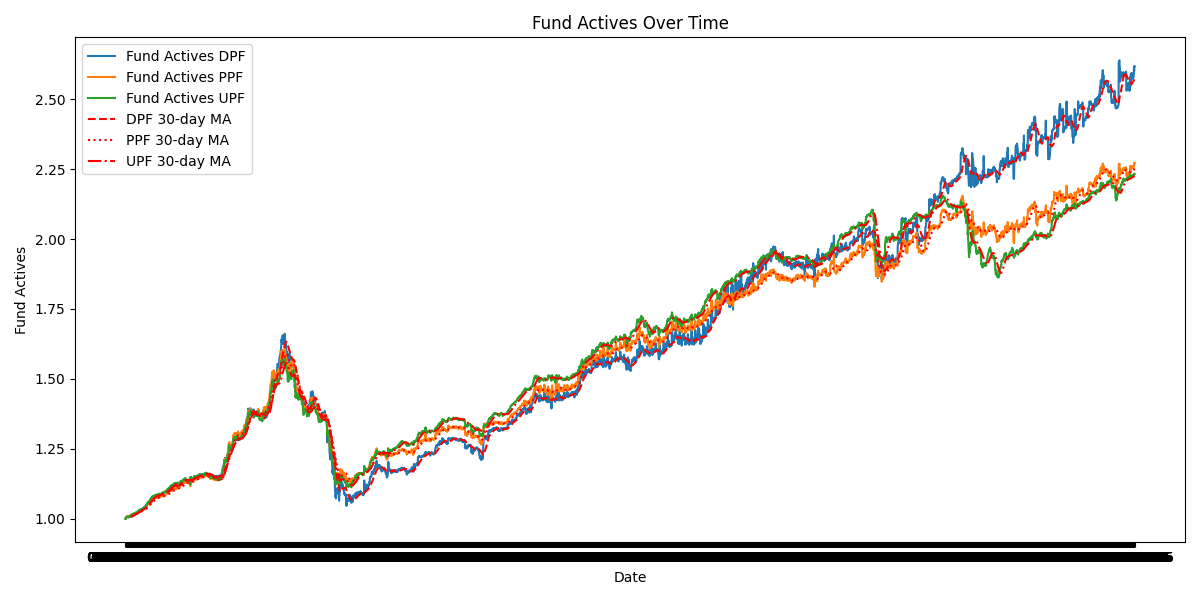
\includegraphics[width=0.8\textwidth]{images/asset_values.png}
        \caption{Стойности на активите на пенсионен фонд "Съгласие" във времето}
        \label{fig:asset_values}
\end{figure}
Можем да използваме библиотеката и за симулация на бъдещи стойности на активите, което може да помогне при вземането на решения относно общият капитал, който лицето ще има при пенсиониране.

\begin{figure}[ht]
        \centering
        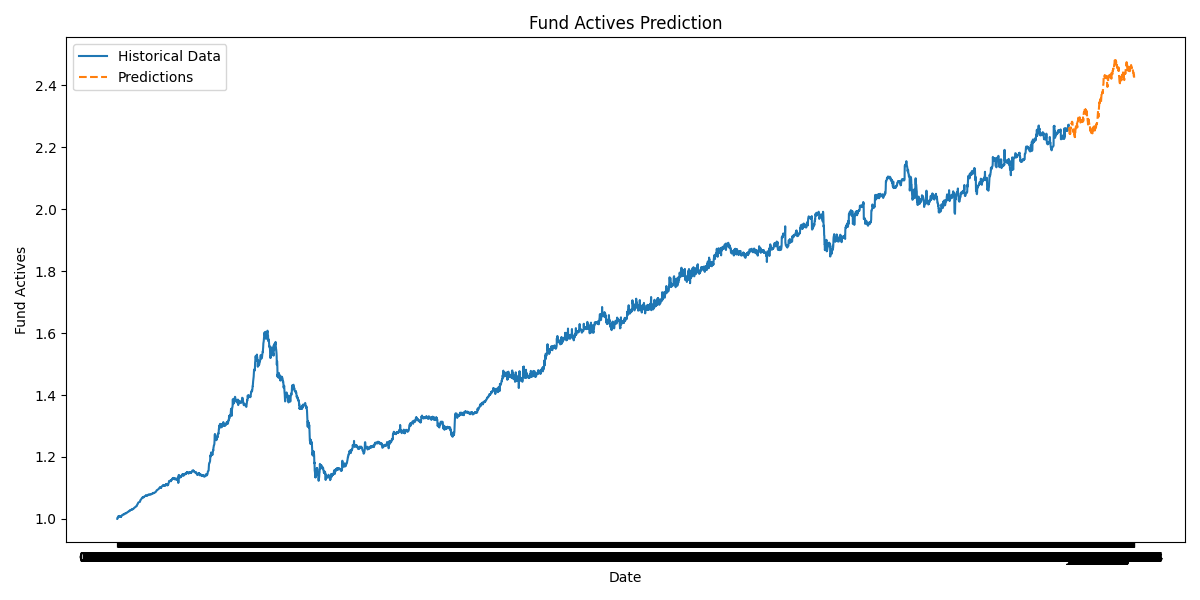
\includegraphics[width=0.8\textwidth]{images/simulated_asset_values.png}
        \caption{Симулация на бъдещи стойности на активите на пенсионен фонд "Съгласие"}
        \label{fig:simulated_asset_values}
\end{figure}
Във фигура \ref{fig:simulated_asset_values} се вижда примерен симулиран път на бъдещите стойности на активите, което дава представа за възможен сценарий в развитието на спестяванията на Георги. Такава симулация се използва при изчислението на стойността на портфейла му при пенсиониране.


\newpage
\section{Заключение}
В заключение, разработената библиотека за пенсионни актюерски изчисления в Python предоставя гъвкав и модерен инструмент за анализ и управление на пенсионните системи.

Тя обединява теоретичните основи на актюерската математика с предимствата на съвременните програмни среди, което я прави подходяща както за академични изследвания, така и за практическо приложение в индустрията. Чрез използването на популярни библиотеки като NumPy, Pandas и Matplotlib, библиотеката осигурява мощни възможности за числени изчисления, обработка на данни и визуализация. Това позволява на потребителите да извършват сложни актюерски изчисления, да анализират финансови данни и да симулират бъдещи сценарии с лекота.

Примерният случай на лице, което се осигурява в пенсионен фонд "Съгласие", демонстрира как библиотеката може да бъде използвана за изчисляване на различни видове пенсии и анализ на финансовите данни. Резултатите показват различните възможности за пенсиониране, които лицето може да избере, в зависимост от неговите нужди и предпочитания. Освен това, анализът на активите на пенсионен фонд "Съгласие" и симулацията на бъдещи стойности предоставят ценна информация за вземане на решения относно управлението на пенсионните спестявания.

\section{Бъдещи разработки}
В бъдеще библиотеката може да бъде разширена с допълнителни функционалности, които да я направят още по-полезна за анализ и сравнение на различни сценарии. Сред основните направления за развитие са:

\begin{itemize}
        \item \textbf{Сравнение между различни пенсионни компании:} Добавяне на възможност за едновременно анализиране и сравняване на условията, лихвените проценти, рисковите параметри и историческите резултати на различни пенсионни дружества. Това ще позволи на потребителите да вземат по-информирани решения при избор на пенсионен фонд.
        \item \textbf{Сравнение между различни участници:} Въвеждане на функционалност за сравнение на пенсиите, спестяванията и финансовите резултати на различни лица с различни демографски и икономически характеристики. Така могат да се анализират ефектите от възраст, доход, стаж и други фактори върху размера на пенсията.
        \item \textbf{Разширени визуализации:} Добавяне на интерактивни графики и таблични сравнения, които да представят резултатите от различните сценарии по ясен и достъпен начин.
        \item \textbf{Интеграция с външни бази данни:} Възможност за автоматично извличане и актуализиране на данни за смъртност, доходи и активи от официални източници.
        \item \textbf{Моделиране на алтернативни пенсионни продукти:} Имплементиране на допълнителни видове пенсии и финансови продукти, които да отразяват разнообразието на пазара.
\end{itemize}

Тези бъдещи разработки ще направят библиотеката още по-гъвкава и приложима както за индивидуални потребители, така и за компании и институции, които желаят да анализират и оптимизират пенсионните си стратегии.
\begin{thebibliography}{99}
        \bibitem{dalriada2023}
        Dalriada Trustees. (2023).
        \emph{The Importance of Mathematics in Pensions}.
        Retrieved from: \url{https://www.dalriadatrustees.co.uk/the-importance-of-mathematics-in-pensions/}

        \bibitem{milliman2022}
        Milliman. (2022).
        \emph{Using Python as an Actuarial Modelling Platform}.
        Retrieved from: \url{https://www.milliman.com/en/insight/using-python-actuarial-modelling-platform}

        \bibitem{bostonfed1999}
        Boston Federal Reserve Bank. (1999).
        \emph{Demographic Trends and Their Impact on Public Pension Systems}.
        Retrieved from: \url{https://www.bostonfed.org/publications/working-papers/1999/demographic-trends-public-pensions.aspx}

        \bibitem{ncpers2023}
        National Conference on Public Employee Retirement Systems (NCPERS). (2023).
        \emph{The Impact of Demographic Shifts on Public Pensions (And What They Can Do About It)}.
        Retrieved from: \url{https://www.ncpers.org/blog_home.asp?display=377}

        \bibitem{lifelib2024}
        Binette, O. (2024).
        \emph{lifelib: Actuarial Models in Python}.
        Retrieved from: \url{https://lifelib.io/}

        \bibitem{hyperexponential2023}
        Hyperexponential. (2023).
        \emph{Python for Insurers and Actuaries}.
        Retrieved from: \url{https://www.hyperexponential.com/blog/python-for-insurance/}

        % Bulgarian Sources
        \bibitem{ZDZPO_2004}
        Народно събрание на Република България. (2004).
        \emph{Закон за допълнителното задължително пенсионно осигуряване}.
        Доставен от: \url{https://www.parliament.bg/bg/laws}

        \bibitem{ZDOO_2000}
        Народно събрание на Република България. (2000).
        \emph{Закон за държавното обществено осигуряване}.
        Доставен от: \url{https://www.parliament.bg/bg/laws}

        \bibitem{DKFN_Pensions}
        Държавна комисия по финансов надзор (ДКФН). (2023).
        \emph{Раздел „Пенсионни фондове“}.
        Доставен от: \url{https://www.dkn.bg}

        \bibitem{NOI_Official}
        Национална осигурителна институция (НОИ). (2023).
        \emph{Официален уебсайт}.
        Доставен от: \url{https://www.noi.bg}

        \bibitem{numpy2024}
        Harris, C. R., Millman, K. J., van der Walt, S. J. et al. (2024).
        \emph{Array programming with NumPy}.
        Nature, 585(7825), 357–362.
        Retrieved from: \url{https://www.numpy.org}

        \bibitem{pandas2024}
        The pandas development team. (2024).
        \emph{pandas-dev/pandas: Pandas}.
        Zenodo.
        Retrieved from: \url{https://pandas.pydata.org}

        \bibitem{matplotlib2024}
        Hunter, J. D., and the Matplotlib development team. (2024).
        \emph{Matplotlib: Visualization with Python}.
        Retrieved from: \url{https://matplotlib.org}

        \bibitem{seaborn2024}
        Waskom, M. L., and the seaborn development team. (2024).
        \emph{Seaborn: statistical data visualization}.
        Journal of Open Source Software, 6(60), 3021.
        Retrieved from: \url{https://seaborn.pydata.org}
\end{thebibliography}
\newpage
\section{Приложения}
\lstinputlisting[language=Python, caption=main.py]{../Code/main.py}
\lstinputlisting[language=Python, caption=company.py]{../Code/Company.py}
\lstinputlisting[language=Python, caption=person.py]{../Code/Person.py}
\lstinputlisting[language=Python, caption=calculator.py]{../Code/Calculator.py}
\lstinputlisting[language=Python, caption=finances.py]{../Code/Finances.py}

\end{document}
